\documentclass[conference]{IEEEtran} % Track A/B: \documentclass[journal]{IEEEtran}. Do not change margins/fonts.
\usepackage{booktabs,graphicx,amsmath,cite,hyperref}
\begin{document}
\title{TITLE}
\author{\IEEEauthorblockN{NAME1, NAME2}\IEEEauthorblockA{FAST-NUCES, Islamabad\\ emails}}
\maketitle
\begin{abstract}
Problem, method, data, main findings (numbers from your final run), implication.
\end{abstract}
\begin{IEEEkeywords}AI-generated text detection, robustness, outreach messages\end{IEEEkeywords}

\section{Introduction}
Context and motivation. \textbf{Gap} (2--3 sentences). \textbf{Novelty} paragraph.
Contributions: (1) Develop \dots{} (2) Evaluate \dots{} (3) Quantify \dots{}
The paper is organised as follows \dots

\section{Literature Review and Hypotheses}
Table~\ref{tab:gap}: 10--15 recent studies, base paper included, last row = proposed work; gaps G1, G2, \dots; hypotheses H1, H2, \dots
\begin{table}[t]\caption{Gap-based comparison of recent studies}\label{tab:gap}\centering
\begin{tabular}{@{}llllll@{}}\toprule
Ref. & Year & Data & Method & Robustness & Gap\\ \midrule
\dots & & & & & \\ \bottomrule\end{tabular}\end{table}

\section{Theoretical Background}
\section{Conceptual Model and Research Design}
% \begin{figure}[t]\centering\includegraphics[width=\columnwidth]{../figures/fig_framework.pdf}\caption{Conceptual framework.}\label{fig:framework}\end{figure}
\section{Base vs Extended Model}
\section{Data and Analysis Setup}
\section{Results and Discussion}
% \begin{figure}[t]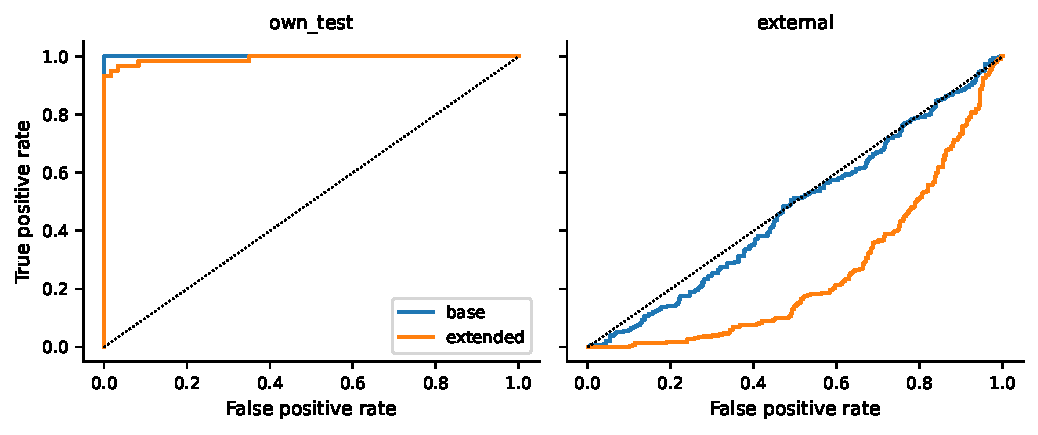
\includegraphics[width=\columnwidth]{../figures/fig_roc.pdf}\caption{ROC curves.}\end{figure}
\section{Robustness Checks}
\section{Practical Implications and Case Study}
\section{Limitations and Future Work}
\section{Conclusion}
\section*{Acknowledgment}
Contributions (CRediT): NAME1: \dots; NAME2: \dots. AI tools were used only for grammar, LaTeX debugging and code debugging.
\bibliographystyle{IEEEtran}
\bibliography{references}
\end{document}
